\documentclass[12pt]{article}
\usepackage{helvet}
\renewcommand{\familydefault}{\sfdefault}
\usepackage[utf8]{inputenc}
\usepackage[spanish]{babel}
\usepackage[left=2.5cm,right=2.5cm,top=3cm,bottom=3cm]{geometry}
\usepackage{parskip} 
\usepackage{graphicx}
\graphicspath{ {figures/} }
\usepackage{array}
\usepackage{multirow}
\usepackage{blindtext}
\usepackage{titlesec}
\usepackage{hyperref}
\usepackage{longtable}
\usepackage{booktabs}
\usepackage{makecell}
\usepackage{pdflscape}
\hypersetup{
    colorlinks,
    citecolor=black,
    filecolor=black,
    linkcolor=black,
    urlcolor=black
}
\pdfgentounicode=1

\usepackage{fancyhdr}
\usepackage{lastpage}
\setlength{\headheight}{2cm}
\renewcommand{\headrulewidth}{0pt}
\renewcommand{\footrulewidth}{0pt}
\pagestyle{fancy}
\lhead{%
    \fbox{%
        \begin{minipage}[t][2cm][c]{.23\linewidth}%
            \begin{center}              
                \includegraphics[width=2.5cm]{Logo.jpeg}             
                CONTRATO No:
            \end{center}
        \end{minipage}%
    }% end \fbox
}% end \lhead

\chead{%
    \fbox{%
        \begin{minipage}[t][2cm][c]{.5\linewidth}%
            \begin{center}
                \textbf{Informe}\\
                \textbf{Nombre de la consultoría, proyecto,etc.}\\
                \textbf{NOMBRE DEL ESTUDIO QUE SE PRESENTA EN ESTE DOCUMENTO.}\\
            \end{center}
        \end{minipage}%
    }% end \fbox
}% end \chead

\rhead{%
    \fbox{%
        \begin{minipage}[t][2cm][c]{.23\linewidth}%
            \begin{center}
                \textbf{Revisión: 1}\\
                \vspace{5mm}
                \textbf{Página \thepage{} de \pageref{LastPage}}
            \end{center}
        \end{minipage}%
    }% end \fbox
}% end \rhead

\begin{document}

\begin{center}
\phantom{This text will be invisible} \\
\vspace{1.5cm}
Informe N°XX\\
Nombre de la asesoría, consultoría, proyecto, etc.\\
\vspace{4cm}
NOMBRE DEL ESTUDIO QUE SE PRESENTA EN ESTE DOCUMENTO.\\
\vspace{4cm}
Elaborado por:\\
Dairo Alexander Lobo Moreno\\
Daniel Fernando Aranda Contreras\\
Yulieth Valentina Portilla Jaimes\\

\vspace{4cm}
Dependencia que desarrolla el informe\\
PROELCO\\
Bucaramanga, 23 de Febrero de 2023.\\
\vspace{2cm}
\end{center}
\newpage
\phantom{This text will be invisible} \\

\begin{table}[h]
\centering
\begin{tabular}{|ccc|}
\hline
\multicolumn{3}{|c|}{ÍNDICE DE REVISIONES}                                                       \\ \hline
\multicolumn{1}{|c|}{Índice revisión} & \multicolumn{1}{c|}{Fecha modificación} & Modificaciones \\ \hline
\multicolumn{1}{|c|}{0}               & \multicolumn{1}{c|}{}                   &                \\ \hline
\multicolumn{1}{|c|}{1}               & \multicolumn{1}{c|}{}                   &                \\ \hline
\end{tabular}
\end{table}

\begin{table}[h]
\centering
\begin{tabular}{|cc|c|c|}
\hline
\multicolumn{2}{|c|}{Versión}                            & 0 & 1 \\ \hline
\multicolumn{1}{|c|}{\multirow{2}{*}{Ejecuta}}  & Nombre &   &   \\ \cline{2-4} 
\multicolumn{1}{|c|}{}                          & Fecha  &   &   \\ \hline
\multicolumn{1}{|c|}{\multirow{2}{*}{Revisa}}   & Nombre &   &   \\ \cline{2-4} 
\multicolumn{1}{|c|}{}                          & Fecha  &   &   \\ \hline
\multicolumn{1}{|c|}{\multirow{2}{*}{Verifica}} & Nombre &   &   \\ \cline{2-4} 
\multicolumn{1}{|c|}{}                          & Fecha  &   &   \\ \hline
\multicolumn{1}{|c|}{\multirow{2}{*}{Aprueba}}  & Nombre &   &   \\ \cline{2-4} 
\multicolumn{1}{|c|}{}                          & Fecha  &   &   \\ \hline
\end{tabular}
\end{table}

\newpage
\vspace*{0.1cm}

\renewcommand\contentsname{Tabla de contenido}
\tableofcontents


\newpage
\vspace*{0.1cm}

\renewcommand{\listfigurename}{Lista de figuras}
\listoffigures


\newpage
\vspace*{0.1cm}

\renewcommand{\listtablename}{Lista de tablas}
\listoftables


\newpage
\vspace*{0.1cm}

\section{Resumen ejecutivo}

\section{Objetivo}
Evaluar el comportamiento eléctrico y la viabilidad técnica de la integración de las Etapas N°1 y N°2 del proyecto "Construcción del Segmento de Potencia del Área Santander" al Sistema Interconectado Nacional (SIN)
, mediante la simulación de flujos de potencia y el análisis de corrientes de falla bajo escenarios de demanda mínima, media y máxima
, con el fin de diagnosticar la regulación de tensión, cuantificar los niveles de cortocircuito en las nuevas subestaciones (Piedecuesta 115 kV, Mesa del Sol 115 kV, San Gil 115 kV, Cabrera 115 kV, Oiba 115 kV, Suaita 115 kV, Barbosa 115 kV y Cabrera 220 kV)
 y determinar el impacto operativo y los aportes de falla sobre los nodos existentes y subestaciones adyacentes del área de influencia (tales como Guatiguará 220 kV y Piedecuesta 220 kV).
\section{Alcance}

El presente estudio técnico, correspondiente a la fase de análisis eléctricos de soporte para el Estudio de Ajuste y Coordinación de Protecciones (EACP), comprende la modelación y evaluación de las condiciones operativas para la integración progresiva de las Etapas N.° 1 y N.° 2 del proyecto de expansión del Área Santander al Sistema Interconectado Nacional (SIN). Empleando un modelo de red ajustado a las condiciones de operación del SIN, la delimitación del área de influencia parte de las barras adyacentes a los puntos de conexión del proyecto, extendiéndose o contrayéndose de acuerdo con los criterios de influencia eléctrica definidos por el Consejo Nacional de Operación (CNO).

En esta fase se ejecutarán los estudios de flujo de carga y cortocircuito para las configuraciones de red de cada etapa. El análisis de flujo de carga permitirá evaluar los perfiles de tensión y la cargabilidad de los elementos para identificar restricciones operativas y, ante desviaciones de la regulación de tensión, establecer la necesidad y las características de la compensación reactiva requerida. Por su parte, el estudio de cortocircuito comprende el cálculo de corrientes de falla para cortocircuitos francos (\(0\,\Omega\)) de tipo monofásico, bifásico a tierra, bifásico y trifásico, bajo los escenarios de demanda máxima y mínima definidos para el estudio..

Los resultados obtenidos constituirán los insumos técnicos para la posterior revisión, ajuste y coordinación de los sistemas de protección asociados a los elementos nuevos, reconfigurados o impactados por el proyecto, incluyendo las líneas de transmisión a 115 kV y 220 kV, el transformador Cabrera 220/115 kV y las instalaciones asociadas a las subestaciones de frontera Piedecuesta, Barbosa y Guatiguará. En consecuencia, esta fase se limita a los estudios de soporte de flujo de carga y cortocircuito, por lo que no comprende la parametrización final de relés ni las verificaciones detalladas de selectividad, las cuales serán desarrolladas en las etapas posteriores del EACP.

\section{Documentos consultados}


\space

\section{Descripción del proyecto}

\subsection{Etapas del proyecto}
El proyecto de expansión de la red de transmisión del Área Santander se desarrolla en 
\textbf{dos etapas de puesta en servicio}, mediante la incorporación progresiva de nueva 
infraestructura al sistema de potencia. Para cada etapa se describe la infraestructura 
prevista y se presenta su respectiva configuración topológica.

\textbf{Etapa N.° 1.} La Etapa N.° 1 comprende la incorporación de la infraestructura 
de transmisión a 115 kV conformada por los enlaces Piedecuesta 115 kV--Mesa del Sol 
115 kV, Mesa del Sol 115 kV--San Gil 115 kV, San Gil 115 kV--Cabrera 115 kV, Cabrera 
115 kV--Oiba 115 kV, Oiba 115 kV--Suaita 115 kV y Suaita 115 kV--Barbosa 115 kV. 
Adicionalmente, contempla la conexión entre Cabrera 115 kV y Cabrera 220 kV mediante 
el transformador de potencia correspondiente.

\textbf{Fecha esperada de entrada en operación:} 22 de abril de 2026.

La configuración topológica correspondiente a esta etapa se presenta en la 
Figura~\ref{fig:etapa1}.
\begin{figure}[!ht]
    \centering
    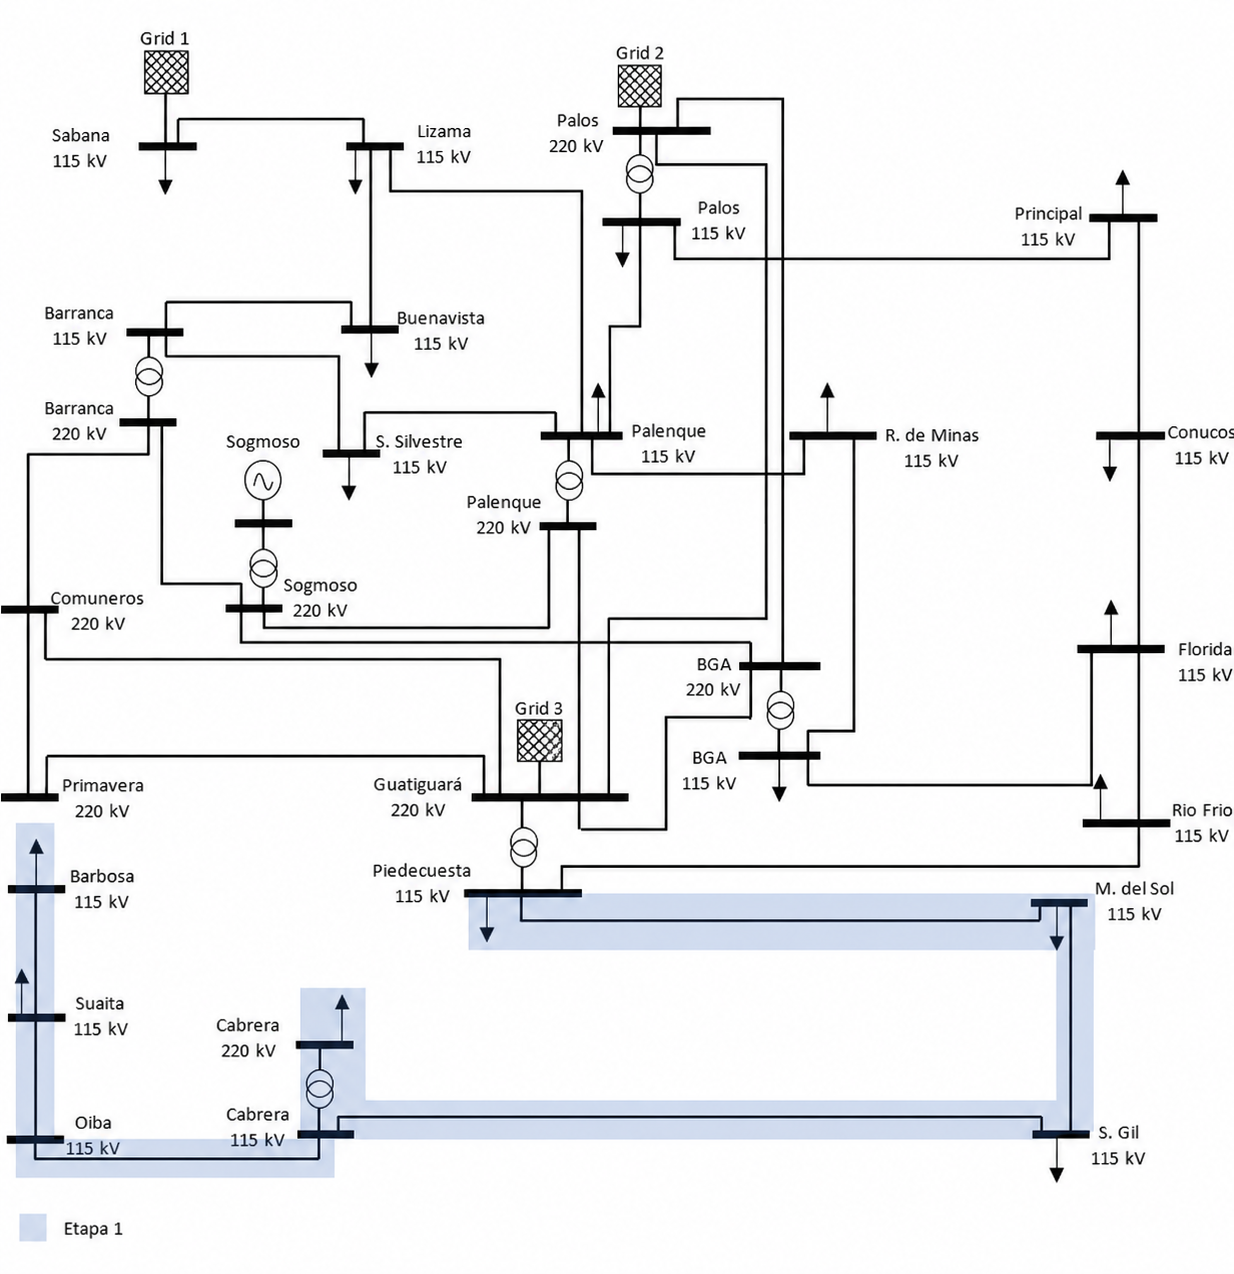
\includegraphics[width=\linewidth]{etapa1.png}
    \caption{Sistema de potencia en estudio: Etapa N.° 1.}
    \label{fig:etapa1}
\end{figure}

\textbf{Etapa N.° 2.} La Etapa N.° 2 comprende la infraestructura incorporada durante 
la Etapa N.° 1 y adiciona el enlace de transmisión Cabrera 220 kV--Guatiguará 220 kV. 
Esta conexión constituye la infraestructura adicional prevista para la segunda etapa 
del proyecto.

\textbf{Fecha esperada de entrada en operación:} 22 de abril de 2027.

La configuración topológica correspondiente a esta etapa se presenta en la 
Figura~\ref{fig:etapa2}.

\begin{figure}[!ht]
    \centering
    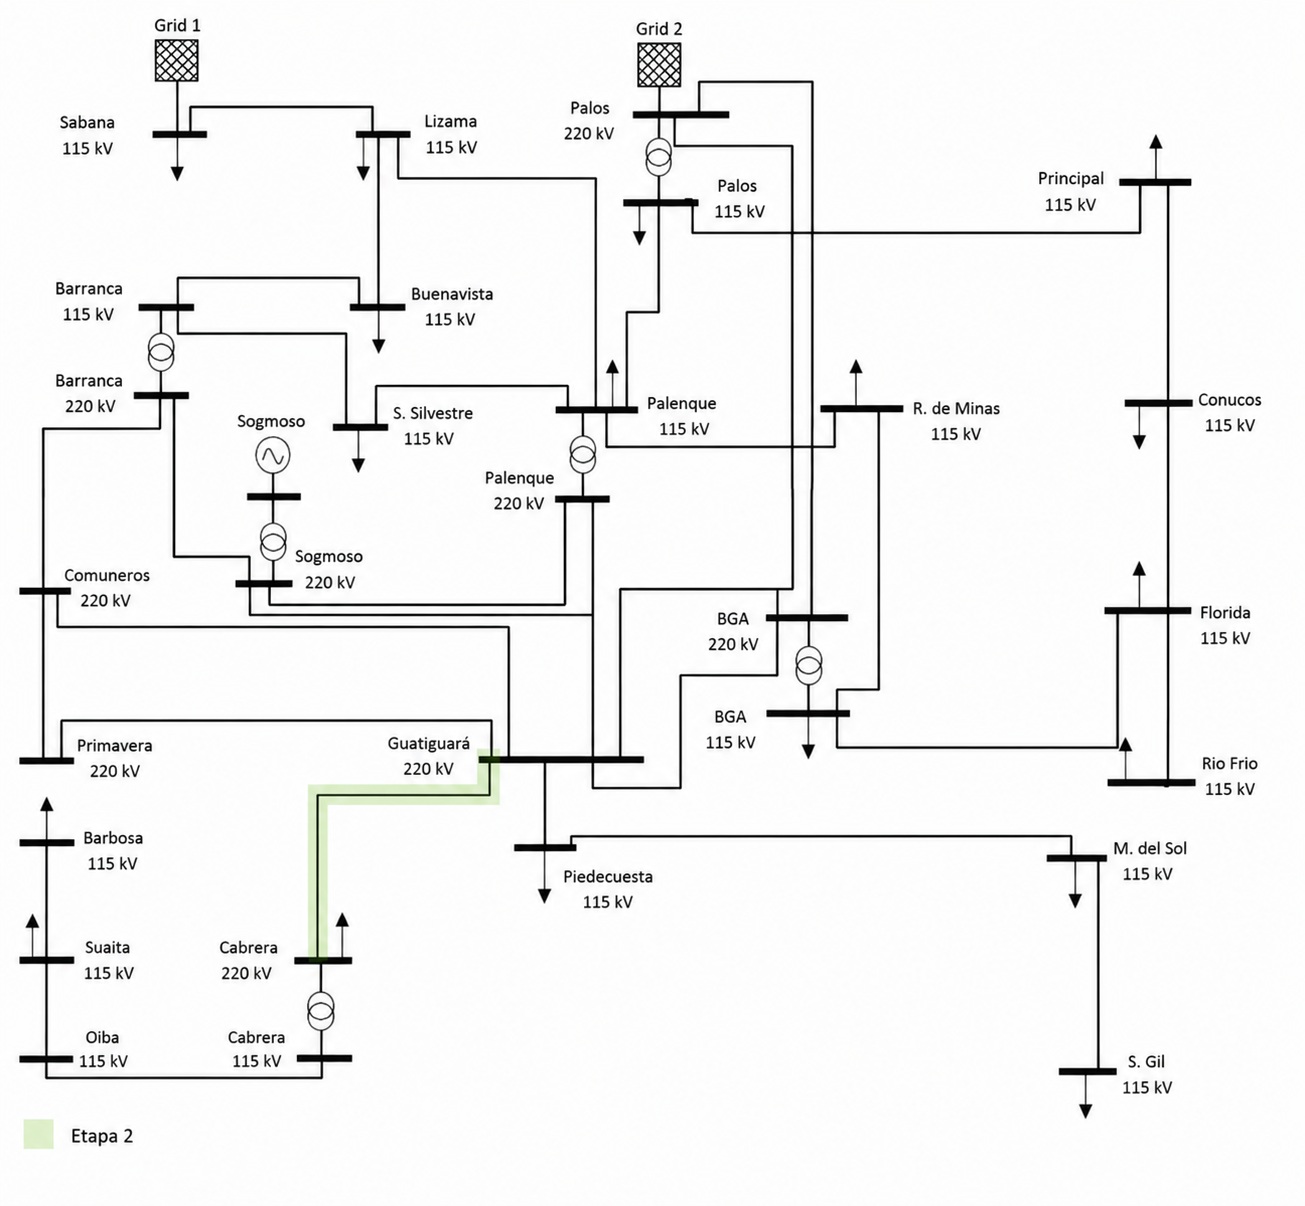
\includegraphics[width=\linewidth]{etapa2.png}
    \caption{Sistema de potencia en estudio: Etapa N.° 2.}
    \label{fig:etapa2}
\end{figure}

\subsection{Ubicación geográfica}

\subsection{Área de influencia}
Para el desarrollo del proyecto se establecen dos áreas de influencia, correspondientes a cada una de las etapas de implementación del proyecto, de acuerdo con la configuración de la red mostrada en los diagramas unifilares.

\textbf{Etapa N.° 1:}

El área de influencia comprende las subestaciones \textbf{Piedecuesta 115 kV, Mesa del Sol 115 kV, San Gil 115 kV, Cabrera 115 kV, Oiba 115 kV, Suaita 115 kV y Barbosa 115 kV}, así como los elementos de transmisión asociados a su interconexión y la conexión entre \textbf{Cabrera 115 kV y Cabrera 220 kV}. Asimismo, se consideran los transformadores de potencia asociados a las subestaciones que hacen parte de la red bajo estudio, teniendo en cuenta su configuración y su incidencia en los análisis de cortocircuito y coordinación de protecciones.

\textbf{Etapa N.° 2:}

El área de influencia comprende la totalidad de la red considerada en la Etapa N.° 1 y se amplía con la incorporación de los elementos asociados a la conexión de \textbf{Cabrera 220 kV con Guatiguará 220 kV}. En esta etapa se incluyen las subestaciones y elementos de transmisión involucrados en dicha integración, junto con los transformadores de potencia correspondientes, de acuerdo con la configuración mostrada en el diagrama unifilar.

Las áreas de influencia definidas para cada etapa se presentan en los \textbf{diagramas unifilares del sistema bajo estudio}, en los cuales se identifican los elementos considerados para el desarrollo de los estudios de flujo de carga, cortocircuito y coordinación de protecciones.

\textbf{Figura X. Área de influencia del EACP -- Etapa N.° 1.}

\textbf{Figura X. Área de influencia del EACP -- Etapa N.° 2.}


\section{Parámetros técnicos}

\subsection{Parámetros de equipos}
\subsubsection{Parámetros de líneas de transmisión}


\begin{center}
\small
\setlength{\tabcolsep}{2pt}
\renewcommand{\arraystretch}{1.15}

\begin{longtable}{|p{5.8cm}|r|r|r|r|r|r|r|r|r|}
\caption{Parámetros técnicos de líneas}
\label{tab:parametros_lineas} \\

\hline
\textbf{Línea} &
\makecell{\textbf{Long.}\\\textbf{[km]}} &
\makecell{\textbf{$R_1$}\\\textbf{[$\Omega$/km]}} &
\makecell{\textbf{$X_1$}\\\textbf{[$\Omega$/km]}} &
\makecell{\textbf{$R_0$}\\\textbf{[$\Omega$/km]}} &
\makecell{\textbf{$X_0$}\\\textbf{[$\Omega$/km]}} &
\makecell{\textbf{$B_0$*}\\\textbf{[S/km]}} &
\makecell{\textbf{$B_1$*}\\\textbf{[S/km]}} &
\makecell{\textbf{$I_{\mathrm{Nom.}}$}\\\textbf{[A]}} &
\makecell{\textbf{$I_{\mathrm{Emerg.}}$}\\\textbf{[A]}} \\
\hline
\endfirsthead

\hline
\multicolumn{10}{|c|}{\textit{Tabla \thetable{} -- continuación}} \\
\hline

\textbf{Línea} &
\makecell{\textbf{Long.}\\\textbf{[km]}} &
\makecell{\textbf{$R_1$}\\\textbf{[$\Omega$/km]}} &
\makecell{\textbf{$X_1$}\\\textbf{[$\Omega$/km]}} &
\makecell{\textbf{$R_0$}\\\textbf{[$\Omega$/km]}} &
\makecell{\textbf{$X_0$}\\\textbf{[$\Omega$/km]}} &
\makecell{\textbf{$B_0$}\textsuperscript{*}\\\textbf{[S/km]}} &
\makecell{\textbf{$B_1$}\textsuperscript{*}\\\textbf{[S/km]}} &
\makecell{\textbf{$I_{\mathrm{Nom.}}$}\\\textbf{[A]}} &
\makecell{\textbf{$I_{\mathrm{Emerg.}}$}\\\textbf{[A]}} \\
\hline
\endhead

\hline
\multicolumn{10}{|r|}{\textit{Continúa en la siguiente página}} \\
\hline
\endfoot

\hline
\endlastfoot

\hline
\endlastfoot

Barranca - Buenavista 115 kV & 12.10 & 0.1934 & 0.4132 & 0.3413 & 1.2579 & 0 & 0 & 530 & 662.50 \\
\hline
Buenavista - Lizama 115 kV & 36.50 & 0.1932 & 0.4126 & 0.3405 & 1.2562 & 0 & 0 & 530 & 662.50 \\
\hline
Lizama - Sabana 115 kV & 33.10 & 0.1622 & 0.4127 & 0.3100 & 1.2332 & 0 & 0 & 240 & 300.00 \\
\hline
Lizama - Palenque 115 kV & 45.60 & 0.1934 & 0.4132 & 0.3410 & 1.2575 & 0 & 0 & 530 & 662.50 \\
\hline
Palenque - S. Silvestre 115 kV & 80.20 & 0.1792 & 0.4783 & 0.8676 & 1.3173 & 0 & 0 & 480 & 600.00 \\
\hline
Barranca - S. Silvestre 115 kV & 8.60 & 0.1872 & 0.4919 & 0.3640 & 1.4965 & 0 & 0 & 530 & 662.50 \\
\hline
Barranca - Sogamoso 220 kV & 52.56 & 0.0797 & 0.4882 & 0.2546 & 1.3900 & 0 & 0 & 900 & 1125.00 \\
\hline
Barranca - Comuneros 220 kV & 10.90 & 0.0725 & 0.5349 & 0.4202 & 1.3450 & 0 & 0 & 810 & 1011.25 \\
\hline
Comuneros - Primavera 220 kV & 111.60 & 0.0705 & 0.5515 & 0.3531 & 1.5300 & 0 & 0 & 810 & 1012.50 \\
\hline
Comuneros - Guatiguará 220 kV & 95.20 & 0.0525 & 0.4749 & 0.2090 & 1.0298 & 0 & 0 & 810 & 1012.50 \\
\hline
Primavera - Guatiguará 220 kV & 162.90 & 0.0543 & 0.4767 & 0.2659 & 1.2971 & 0 & 0 & 980 & 1225.00 \\
\hline
Guatiguará - Palenque 220 kV & 45.00 & 0.0513 & 0.4882 & 0.2227 & 1.7271 & 0 & 0 & 1000 & 1250.00 \\
\hline
Palenque - Palos 115 kV & 10.70 & 0.1925 & 0.4907 & 0.3701 & 1.4935 & 0 & 0 & 530 & 662.50 \\
\hline
Palos - Guatiguará 220 kV & 30.60 & 0.0614 & 0.4837 & 0.2781 & 1.1971 & 0 & 0 & 840 & 1050.00 \\
\hline
Guatiguará - Bucaramanga 220 kV & 12.11 & 0.0710 & 0.5120 & 0.3939 & 1.3592 & 0 & 0 & 840 & 1050.00 \\
\hline
Sogamoso - Palenque 220 kV & 40.00 & 0.0512 & 0.4883 & 0.2225 & 1.7270 & 0 & 0 & 1000 & 1250.00 \\
\hline
Sogamoso - Bucaramanga 220 kV & 44.70 & 0.0801 & 0.4911 & 0.2559 & 1.3980 & 0 & 0 & 900 & 1125.00 \\
\hline
Palenque - Real de Minas 115 kV & 5.12 & 0.2129 & 0.4980 & 0.3594 & 1.3359 & 0 & 0 & 530 & 662.50 \\
\hline
Real de Minas - Bucaramanga 115 kV & 8.68 & 0.2281 & 0.4758 & 0.3975 & 1.4309 & 0 & 0 & 530 & 662.50 \\
\hline
Palos - Principal 115 kV & 4.20 & 0.1167 & 0.4500 & 0.3238 & 1.3000 & 0 & 0 & 520 & 650.00 \\
\hline
Principal - Conucos 115 kV & 12.74 & 0.1264 & 0.5118 & 0.3438 & 1.3854 & 0 & 0 & 520 & 650.00 \\
\hline
Conucos - Florida 115 kV & 11.81 & 0.1338 & 0.5368 & 0.3429 & 1.4598 & 0 & 0 & 520 & 650.00 \\
\hline
Florida - Rio Frio 115 kV & 3.60 & 0.1194 & 0.4778 & 0.4722 & 1.3694 & 0 & 0 & 550 & 687.50 \\
\hline
Bucaramanga - Palos 220 kV & 23.45 & 0.0789 & 0.4925 & 0.2546 & 1.5565 & 0 & 0 & 900 & 1125.00 \\
\hline
Florida - Bucaramanga 115 kV & 1.74 & 0.1437 & 0.5402 & 0.3218 & 1.5172 & 0 & 0 & 590 & 737.50 \\
\hline
Rio Frio - Piedecuesta 115 kV & 11.95 & 0.1364 & 0.5004 & 0.2711 & 1.0603 & 0 & 0 & 530 & 662.50 \\
\hline
Piedecuesta - Mesa del Sol 115 kV & 20.60 & 0.2126 & 0.5170 & 0.3898 & 1.6272 & 0 & 0 & 1000 & 1250.00 \\
\hline
San Gil- Mesa del Sol 115 kV & 40.00 & 0.2130 & 0.5170 & 0.3900 & 1.6270 & 0 & 0 & 460 & 575.00 \\
\hline
San Gil - Cabrera 115 kV & 6.45 & 0.2129 & 0.5171 & 0.3898 & 1.6279 & 0 & 0 & 460 & 575.00 \\
\hline
Cabrera - Oiba 115 kV & 45.42 & 0.1990 & 0.4833 & 0.3644 & 1.5207 & 0 & 0 & 458 & 572.50 \\
\hline
Cabrera - Guatiguará 220 kV & 63.00 & 0.0502 & 0.4740 & 0.2965 & 1.1675 & 0 & 0 & 1000 & 1250.00 \\
\hline
Suaita - Oiba 115 kV & 25.00 & 0.2128 & 0.5172 & 0.3900 & 1.6272 & 0 & 0 & 460 & 575.00 \\
\hline
Suaita - Barbosa 115 kV & 39.00 & 0.2128 & 0.5172 & 0.3900 & 1.6272 & 0 & 0 & 460 & 575.00 \\

\end{longtable}
\end{center}

\vspace{-0.2cm}
\begin{flushleft}
\scriptsize
\textit{*} Las susceptancias longitudinales de las líneas se consideran iguales a cero, 
despreciando su efecto debido a la longitud relativamente corta de los tramos analizados.

\textit{**} La corriente de emergencia se estima como el 125\% de la corriente nominal 
de cada línea, es decir, $I_{\mathrm{Emerg.}}=1.25\,I_{\mathrm{Nom.}}$. Esta consideración 
corresponde a una aproximación adoptada para el desarrollo del estudio ante la ausencia 
de información específica sobre las capacidades de emergencia de las líneas.
\end{flushleft}
\subsubsection{Parámetros de generadores}
\begin{center}

\textbf{Cuadro 2: Parámetros técnicos de los generadores}

\vspace{2mm}

\scriptsize
\renewcommand{\arraystretch}{0.95}

\begin{tabular}{|c|c|p{6.0cm}|c|}
\hline

\textbf{Planta} &
\textbf{Unidad de} &
\multicolumn{1}{|c|}{\textbf{Parámetro (*)}} &
\textbf{Valor} \\

&
\textbf{generación} &
&
\\
\hline

\multirow{39}{*}{\centering Sogamoso}
&
\multirow{13}{*}{\centering U1}
& Potencia nominal [MVA] & 324 \\ \cline{3-4}
& & Tensión nominal [kV] & 16,5 \\ \cline{3-4}
& & Corriente nominal [A] & 11\,338 \\ \cline{3-4}
& & Factor de potencia [pu] & --- \\ \cline{3-4}
& & Reactancia Xd saturada [pu] & --- \\ \cline{3-4}
& & Reactancia Xq saturada [pu] & --- \\ \cline{3-4}
& & Reactancia Xd' saturada [pu] & --- \\ \cline{3-4}
& & Reactancia Xq' saturada [pu] & --- \\ \cline{3-4}
& & Reactancia Xd'' saturada [pu] & --- \\ \cline{3-4}
& & Reactancia Xq'' saturada [pu] & --- \\ \cline{3-4}
& & Inercia [s] & --- \\ \cline{3-4}
& & Tipo de puesta a tierra & --- \\ \cline{3-4}
& & Impedancia de la puesta a tierra [$\Omega$] & --- \\ \cline{2-4}

&
\multirow{13}{*}{\centering U2}
& Potencia nominal [MVA] & 324 \\ \cline{3-4}
& & Tensión nominal [kV] & 16,5 \\ \cline{3-4}
& & Corriente nominal [A] & 11\,338 \\ \cline{3-4}
& & Factor de potencia [pu] & --- \\ \cline{3-4}
& & Reactancia Xd saturada [pu] & --- \\ \cline{3-4}
& & Reactancia Xq saturada [pu] & --- \\ \cline{3-4}
& & Reactancia Xd' saturada [pu] & --- \\ \cline{3-4}
& & Reactancia Xq' saturada [pu] & --- \\ \cline{3-4}
& & Reactancia Xd'' saturada [pu] & --- \\ \cline{3-4}
& & Reactancia Xq'' saturada [pu] & --- \\ \cline{3-4}
& & Inercia [s] & --- \\ \cline{3-4}
& & Tipo de puesta a tierra & --- \\ \cline{3-4}
& & Impedancia de la puesta a tierra [$\Omega$] & --- \\ \cline{2-4}

&
\multirow{13}{*}{\centering U3}
& Potencia nominal [MVA] & 324 \\ \cline{3-4}
& & Tensión nominal [kV] & 16,5 \\ \cline{3-4}
& & Corriente nominal [A] & 11\,338 \\ \cline{3-4}
& & Factor de potencia [pu] & --- \\ \cline{3-4}
& & Reactancia Xd saturada [pu] & --- \\ \cline{3-4}
& & Reactancia Xq saturada [pu] & --- \\ \cline{3-4}
& & Reactancia Xd' saturada [pu] & --- \\ \cline{3-4}
& & Reactancia Xq' saturada [pu] & --- \\ \cline{3-4}
& & Reactancia Xd'' saturada [pu] & --- \\ \cline{3-4}
& & Reactancia Xq'' saturada [pu] & --- \\ \cline{3-4}
& & Inercia [s] & --- \\ \cline{3-4}
& & Tipo de puesta a tierra & --- \\ \cline{3-4}
& & Impedancia de la puesta a tierra [$\Omega$] & --- \\ \hline

\end{tabular}

\vspace{3mm}

\begin{minipage}{0.90\textwidth}
\footnotesize
\textit{(*) Para este EACP de líneas, solo se requieren los datos de potencia,
tensión y corriente nominal de los generadores ubicados en el área de
influencia, conforme a los Lineamientos del CNO. La corriente nominal fue
calculada a partir de la potencia y tensión nominal.}
\end{minipage}

\end{center}
\section{Estudio de flujo y cortocircuito}

\subsection{Análisis de flujo}

\subsection{Resultados de cortocircuito}

\subsection{Conclusiones y recomendaciones}


\newpage
\vspace*{0.1cm}

\begin{thebibliography}{1}
\bibliographystyle{IEEEtran}

\bibitem{ref1}
Z. Othman and A. Satria Prabuwono, “Preliminary study on Iris recognition system: Tissues of body organs in iridology,” \emph{2010 IEEE EMBS Conference on Biomedical Engineering and Sciences (IECBES)}, pp. 115–119, Nov. 2010.

\bibitem{ref2}
J. Rojas, “Herramienta Web para el apoyo al diagnóstico de enfermedades en la medicina alternativa a través de la interpretación morfológica del iris del ojo.,” Tesis, Universidad del Valle, Tulúa, 2013.

\bibitem{ref3}
S. P. Jogi and B. B. Sharma, “Methodology of Iris image analysis for clinical diagnosis,” \emph{2014 International Conference on Medical Imaging, m-Health and Emerging Communication Systems (MedCom)}, pp. 235–240, Nov. 2014. 

\bibitem{ref4}
\emph{Information technology - Biometric sample quality - Part 6: Iris image data}, ISO/IEC 29794-6:2015, International Organization for Standardization, ISO, 2015. [En línea]. Disponible: https://www.iso.org/standard/54066.html

\bibitem{ref5}
M. Moncho Santonja, B. Micó-Vicent, B. Defez, J. Jordán, \& G. Peris-Fajarnes, “Hough Transform Sensitivity Factor Calculation Model Applied to the Analysis of Acne Vulgaris Skin Lesions,” \emph{Applied Sciences}, vol. 12, no. 3, pp. 1–12, Feb. 2022. 

\bibitem{ref6}
I. I. Quenta, “Modelo de Diagnostico de Enfermedades Basado en la Iridolgía,” Tesis Doctoral, Universidad Mayor de San Andrés, La Paz, Bolivia, 2009. 

\bibitem{ref7}
Microsoft, “Documentation for visual studio code,” \emph{Visual Studio Code}, 03-Nov-2021. [En línea]. Disponible: https://code.visualstudio.com/docs. [Acceso: 12-Nov-2022]. 

\bibitem{ref8}
Python Software Foundation, “What is python? Executive summary,” \emph{Python}. [En línea]. Disponible: https://www.python.org/doc/essays/blurb/. [Acceso: 12-Nov-2022]. 

\bibitem{ref9}
Python Software Foundation, “Tkinter - Python interface to Tcl/Tk,” \emph{Python}. [En línea]. Disponible: https://docs.python.org/3/library/tkinter.html. [Acceso: 12-Nov-2022]. 

\bibitem{ref10}
Dobeš, M., Martinek J., Skoupil D., Dobešová Z.,  Pospíšil J., “Human eye localization using the modified Hough transform”. \emph{Optik}, vol 117, no. 10, pp. 468-473, Elsevier 2006. ISSN 0030-4026.

\bibitem{ref11}
Dobeš M., Machala L., Tichavský P., Pospíšil J., “Human Eye Iris Recognition Using the Mutual Information”. \emph{Optik}, vol 115, no. 9, pp. 399-405, Elsevier 2004. ISSN 0030-4026.

\bibitem{ref12}
Michal Dobeš and Libor Machala, Iris Database, http://phoenix.inf.upol.cz/iris/

\end{thebibliography}

\newpage
\vspace*{0.1cm}

\section*{Anexo A}

\section*{Anexo B}

\section*{Apéndice A}

\section*{Apéndice B}

\end{document}
